\section{REngine Core}
\subsection{Общие сведения}

REngine Core - трёхмерный графический движок, работающий на базе DirectX 7/8 и совместимый с версиями Windows 2000 и выше. Язык разработки: C/C++.

\subsection{Основные требования к движку}

\begin{itemize}
	\item способен выводить трёхмерную полигональную графику с поддержкой текстур;
	\item поддержка всех трёх осей для свободного позиционирования объектов в пространстве;
	\item события;
	\item возможность управления свободной камерой;
	\item окно;
	\item добавление объектов (obj?) в сцену;
	\item отображение сцены.
\end{itemize}

\subsection{REngine}

\begin{itemize}
	\item поддержка игрока с работающими коллизиями;
	\item поддержка собственного формата уровней - .rem (REngine Map);
	\item визуальный редактор уровней (REditor);
	\item обработка событий.
\end{itemize}

\begin{figure}[ht]
	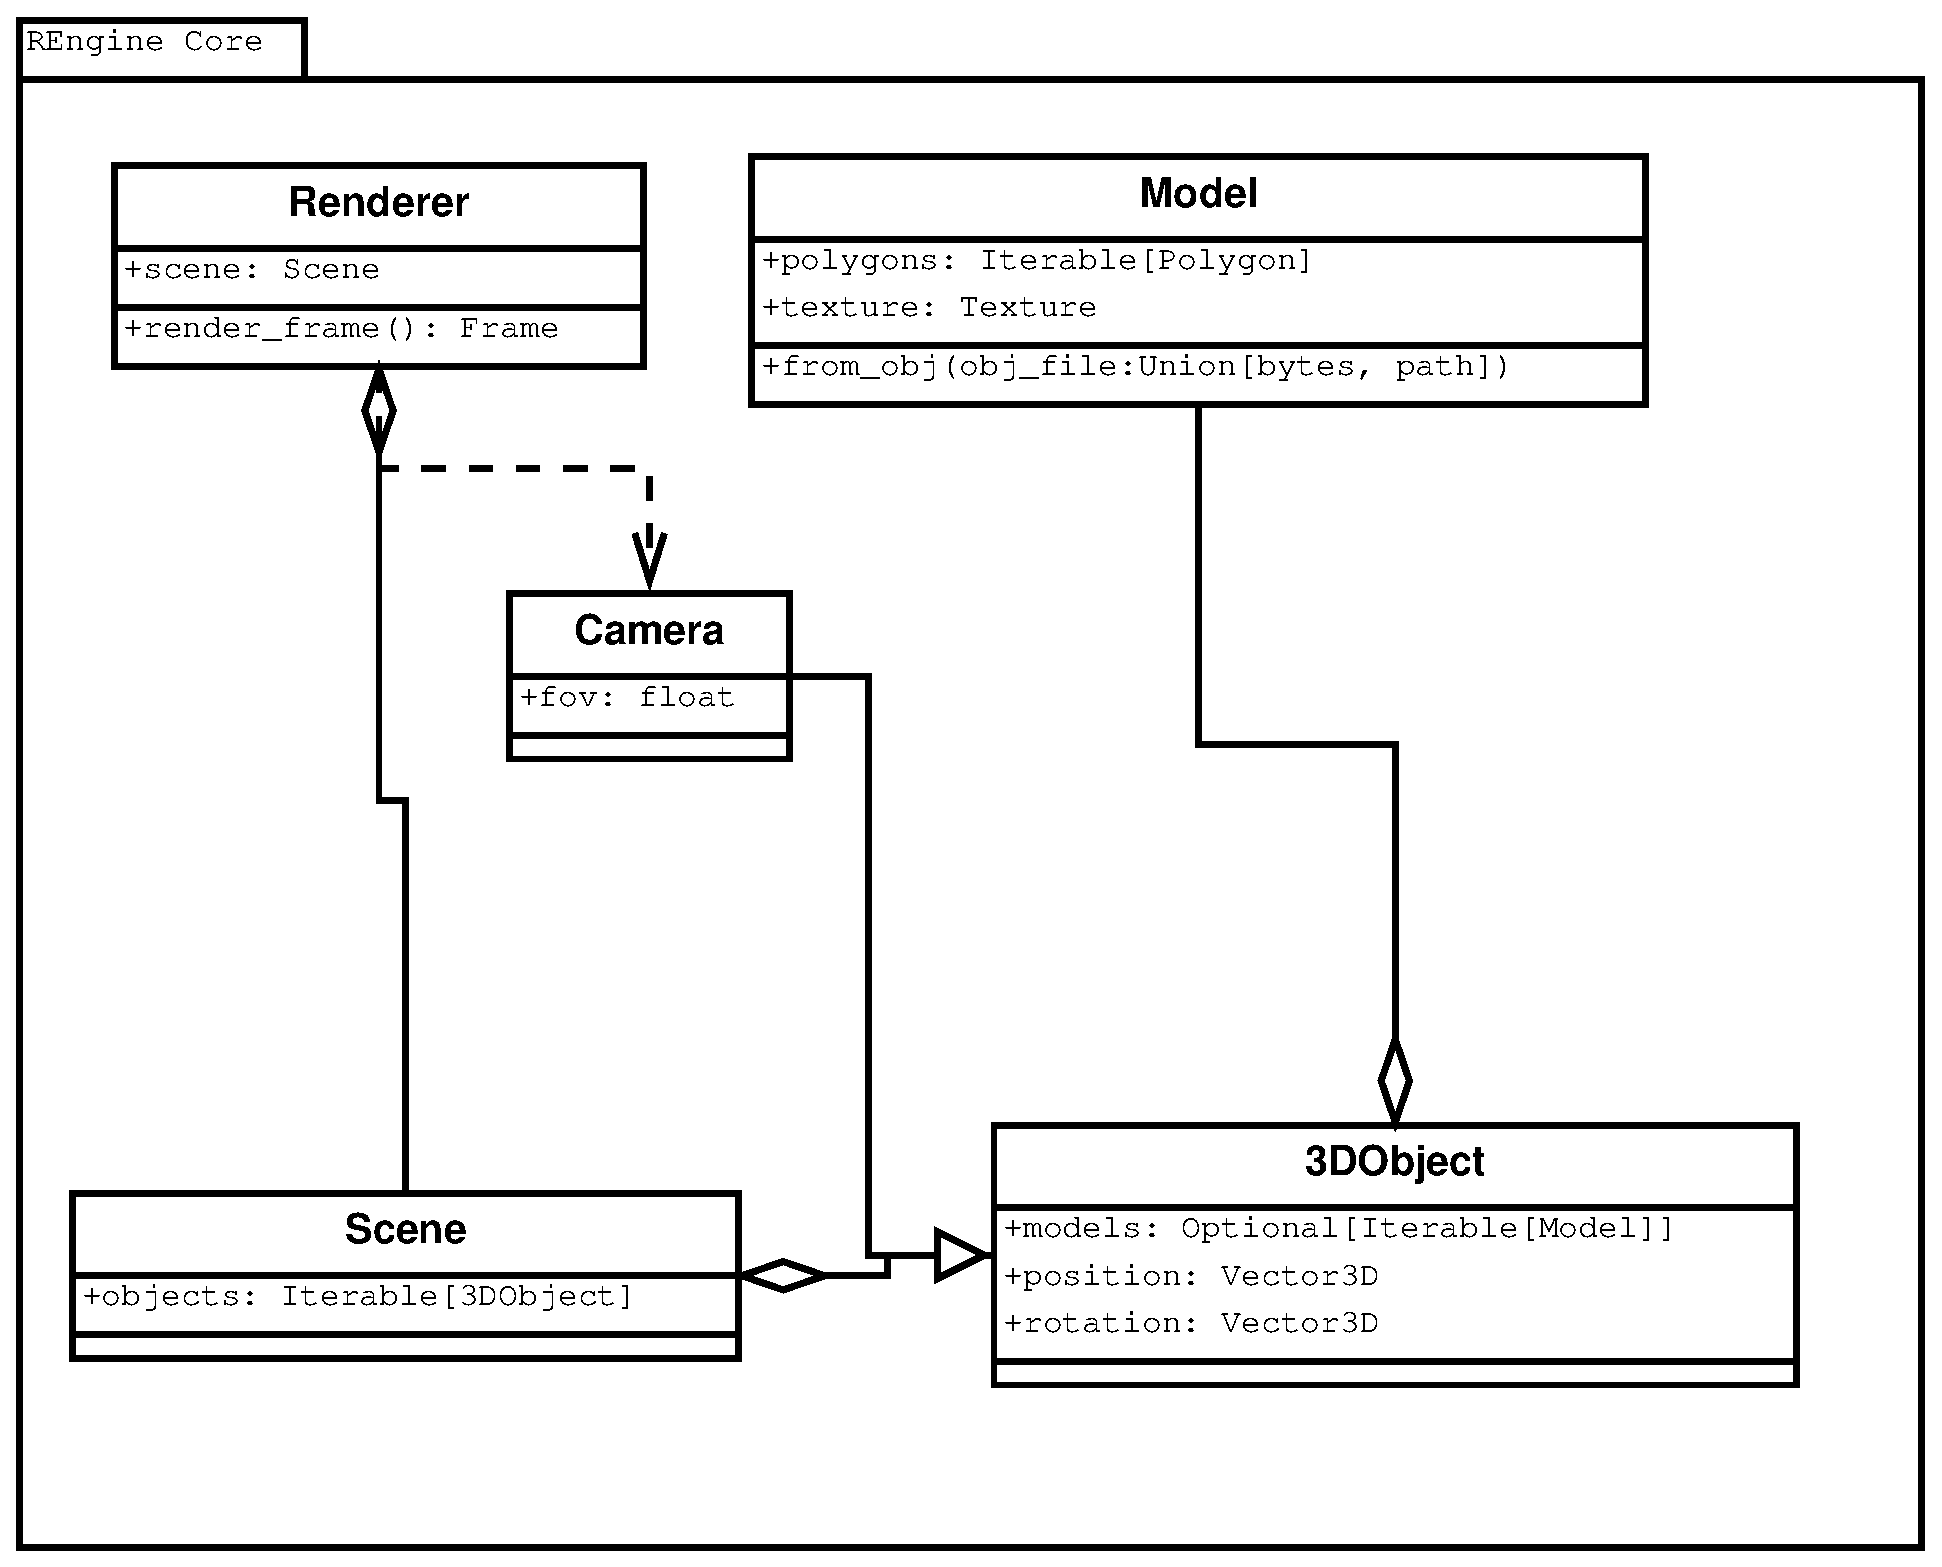
\includegraphics[width=1\linewidth]{architecture}
	\caption{Ранняя архитектура движка}
	\label{architecture:image}
\end{figure}